\chapter{Quality Assurance} \label{cha:qa}
	This chapter explains and describes various quality assurance techniques 
	that were used during the project, to allow us to deliver a product of 
	good quality (regarding both code quality and gameplay quality). It also
	talks a bit about Microsoft Visual Studio first, our IDE of choice for
	this project, considering that some QA tools are not available for
	MonoDevelop, the standard IDE packaged with Unity.
	
	\section{IDE used for programming} \label{sec:ide}
		The IDE used for programming was Microsoft Visual Studio. Unity has an IDE
		of its own available for programming in C\#, which is called MonoDevelop.
		However, the MonoDevelop IDE is really lacking in functionality. It has no
		support for the plugins that we use to check our code. Furthermore, the use
		of MonoDevelop enforces a code style that is incompatible with the style 
		guidelines used by StyleCop (see \ref{sec:codestyle}), 
	
	\section{Testing} \label{sec:testing}
		There are three main types of testing done during the project. These are
		unit testing, integration testing and user testing. Unity has no native
		support for running unit\slash integration tests that have been written,
		but there is a toolkit available for free on the Asset Store, called
		Unity Test Tools,  that does have this support. The extension is
		developed by the Unity team, and can be found on the Unity Asset Store: 
		\url{https://www.assetstore.unity3d.com/en/#!/content/13802}.
		Using this extension, a new menu bar item, called "Unity Test Tools"
		will appear in the main Unity editor. Clicking on this item creates a drop
		down menu with different options, the most important one being the unit test
		runner.
		
		\subsection{C\# Unit Tests} \label{ssec:csharpunittests)}
			Unit tests are written using the NUnit unit testing framework for 
			C\#. NUnit is a test framework which was ported from the Java test 
			framework JUnit, and was created to bring xUnit testing to all .NET 
			languages. Using this framework is also really easy, and a tutorial 
			on how to write unit tests using NUnit can be found using Google. 
			Using Unity Test Tools, all unit tests in the project are listed 
			once one clicks on the subitem "Unit Test Runner". The tests are 
			listed in a new window, and one can run all unit tests by clicking 
			on the "Run All" button at the top. The menu then shows what unit 
			tests have passed or failed, and clicking on a unit test shows what 
			went wrong. A unit testing overview can be seen in \ref{fig:unitytesttools}.
			The UnityTest testing class seen in the overview also displays
			the different statuses of tests in the NUnit framework (passing,
			failing, inconclusive, not executed, and culture specific).
			
			\begin{figure}[!ht]
				\centering
				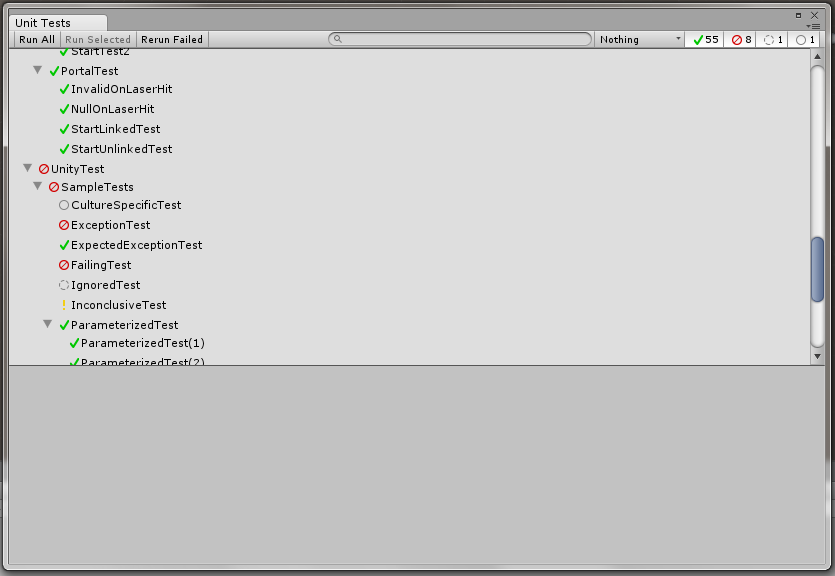
\includegraphics[width=\textwidth]{UnityTestTools}
				\caption{The Unity Test Tools unit testing screen.}
				\label{fig:unitytesttools}
			\end{figure}
			
		\subsection{C++ Unit Tests} \label{ssec:cplusplusunittests}
			The unit tests for the C++ server code are not written using the
			NUnit framework, as that would not really work. The framework for
			the tests in C++ is the Google Test framework. Google test is, like
			NUnit for C\# and JUnit for Java, an xUnit-based testing framework.
			As such, it also supports assertions, type parameterization, etc.
			Also, it is open source, licensed under the new BSD license.
			
            To implement the testing functionality into the server project, 
            the unit tests are separated into their own subproject, which 
            links to the server and runs the tests. As recommended by the 
            Google Test guide, the Google test framework source and headers 
            are included directly into the unit tests subproject, ensuring 
            that the tests can be compiled and run regardless of the platform 
            or compiler being used.

            Because most of the functionality implemented in C++ involves
            computer vision, we've prepared images so that situations can be
            reliably reproduced for test cases. This allows us to test the
            algorithms under many different lighting conditions at once, for
            instance, which saves us a huge amount of time. Some of the tests
            involve functionality that returns an image as result. We've created
            the image we expect and have written utility functions to check if
            two images are approximately equal.
		
		\subsection{Integration Tests} \label{ssec:integrationtests}
			Integration tests are not done via a formalized test procedure, but 
			rather by creating simple scenes and observing that the subjects of 
			the test work as they should when they are placed in an actual 
			scene. It is also a lot harder to run these tests in a standardized 
			way most of the time.

		\subsection{User Tests}
			Although testing the code is important and it helps ensure that the
			software is working correctly, it doesn't tell us anything about the
			actual usability of the product. Since we have been developing a game, 
			it is especially important that the end users will have fun using the
			product. Properties like these can be evaluated by doing user tests.

			Most of the initial play testing has been done by us, the developers,
			because external parties would not have had a good experience while 
			the game was still in the middle of development. However, as the 
			project was nearing completion, the game could no longer be objectively
			played and tested by the developers. At that point, we were already
			too familiar with the levels and game mechanics to be able to properly
			judge if the concepts are too hard to figure out for new players. By 
			having a lot of other people play the game, we were able to estimate if 
			certain levels were either too easy or too hard, and if all of the 
			different game objects were easy to understand and fun to interact with.

			Finding other computer science students to play the game was not much of 
			a problem, but we also needed to have other people play the game, to get 
			a good overview of how different people perceive the game. This is
			especially important, as computer science students mostly indicated the 
			technical issues and limitations of the Meta One glasses, which were mostly
			already known to us.
			
			%TODO Add results of user testing with non-EEMCS students/people.
		
		\subsection{Code coverage} \label{ssec:codecoverage}
			Code coverage is a metric that can be used to determine how thorough
			the written code has been tested. We have to consider generating 
            code coverage reports for two languages: The C\# Unity project and 
            the C++ server project. 
            
            Generating code coverage reports for the C\# code is unexpectedly 
            difficuly: Even though here are several free software packages 
            available on the Internet that allow for generating code
			coverage reports of NUnit test suites, these are hard to use when 
            combined with unit tests in Unity. The reason behind this is that, 
            to run the unit tests for the game, the Unity Test Tools 
            functionality has to be used (as most tests use instantiation of 
            gameplay objects, something that canonly happen in Unity). This 
            functionality has no way of integrating the NCover or OpenCover 
            software packages. It is possible to integrate these with Microsoft 
            Visual Studio, however it is impossible to run the unit tests from 
            that IDE. As such, we had to manually check if the tests tested all 
            possible branches of the code.
            
            On the other hand, however, analysing code coverage for the C++ 
            project is almost trivial: For GNU compilers, including MinGW, 
            there is a utility called gcov, which measures code coverage of 
            GTest-based unit tests. And when using the Microsoft Visual C++ 
            compiler, it is possible to use Visual Studio to analyse the 
            coverage of the unit tests. The tool used for analyzing C++
            code coverage through tests is called OpenCppCoverage, which
            is compatible with Microsoft Visual Studio 2008 and later.
            It easily measures unit test code coverage, and also does not
            require any extra tools to actually generate the report that
            describes the measuring results. These are immediately afterwards
            given in a HTML file. An example of such a report and its results
            is given in \ref{cpppie}, while an example of which lines of code have
            been analyzed is given in \ref{cpplines}.
            
            \begin{figure}[!ht]
            	\centering
            	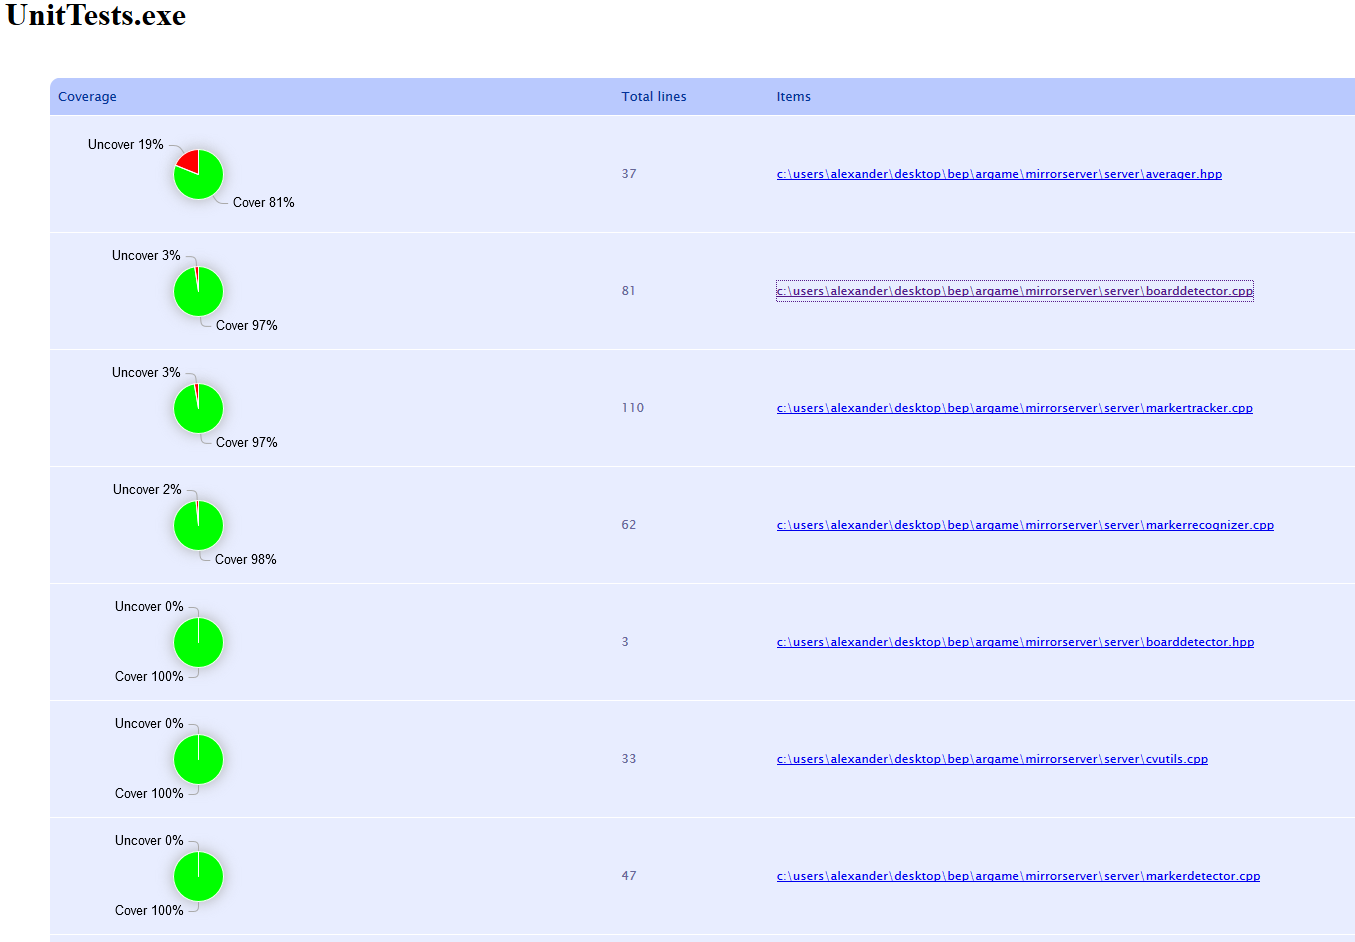
\includegraphics[width=\textwidth]{CPPCoveragePie}
            	\caption{The C++ code coverage report.}
            	\label{fig:cpppie}
            \end{figure}
            
            \begin{figure}[!ht]
                \centering
                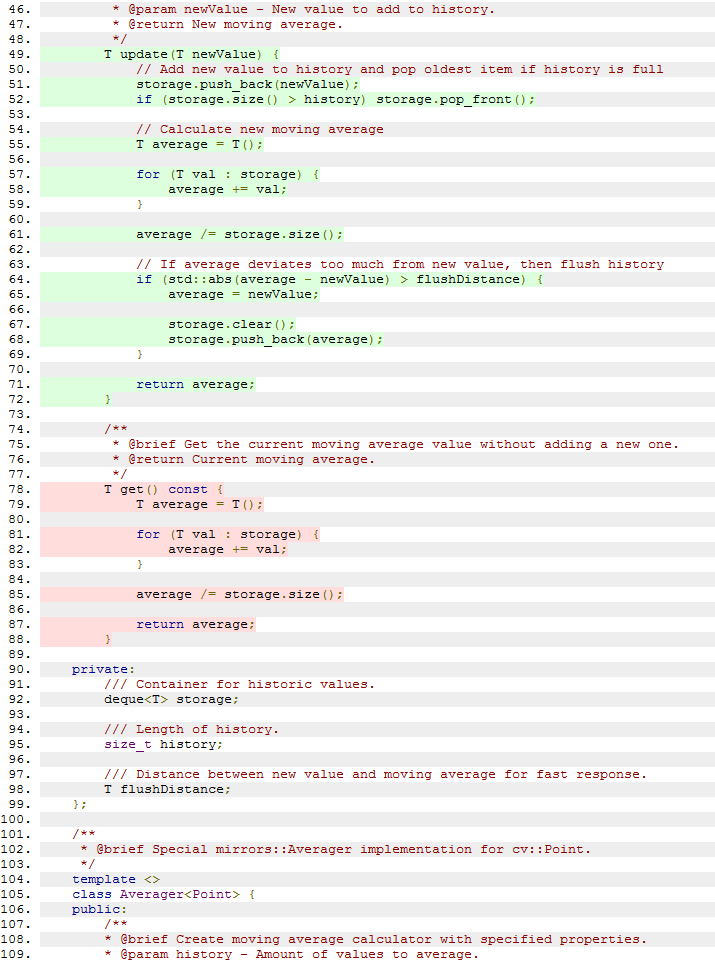
\includegraphics[scale = 0.5]{CPPCoverageLines}
                \caption{The C++ code coverage report, with covered and uncovered lines.}
                \label{fig:cpplines}
            \end{figure}
			
	\section{Code Style} \label{sec:codestyle}
		We decided to stick to the code style guidelines defined by StyleCop and 
		FxCop, two utilities developed by Microsoft. These utilities check for 
		common programming and code style errors in projects so that these can 
		easily be identified and fixed. 
		
		During the project, we kept the source code style checked by periodically
		dedicating time solely for checking code style and performing code 
		maintenance. This also included writing or improving unit tests and 
		refactoring classes and methods with a relatively high complexity or other 
		issues as indicated by StyleCop and FxCop.
		
	\section{SonarQube} \label{sec:sonarqube}
		For getting a clear overview of the source code quality of the project, as 
		well as the issues indicated by FxCop and StyleCop (see section 
		\ref{sec:codestyle}), we made use of a SonarQube server, hosted on one of 
		our development machines. SonarQube keeps track of issues indicated by 
		the abovementioned tools, and performs various code metrics, like cyclomatic 
		complexity and dependency cycles. Using SonarQube enabled us to spot 
		problematic classes and methods and allowed us to improve the overall 
		structure of the source code of the project. An example of a SonarQube
		overview can be seen in figure \ref{fig:sonarqube}
		
		\begin{figure}[!ht]
			\centering
			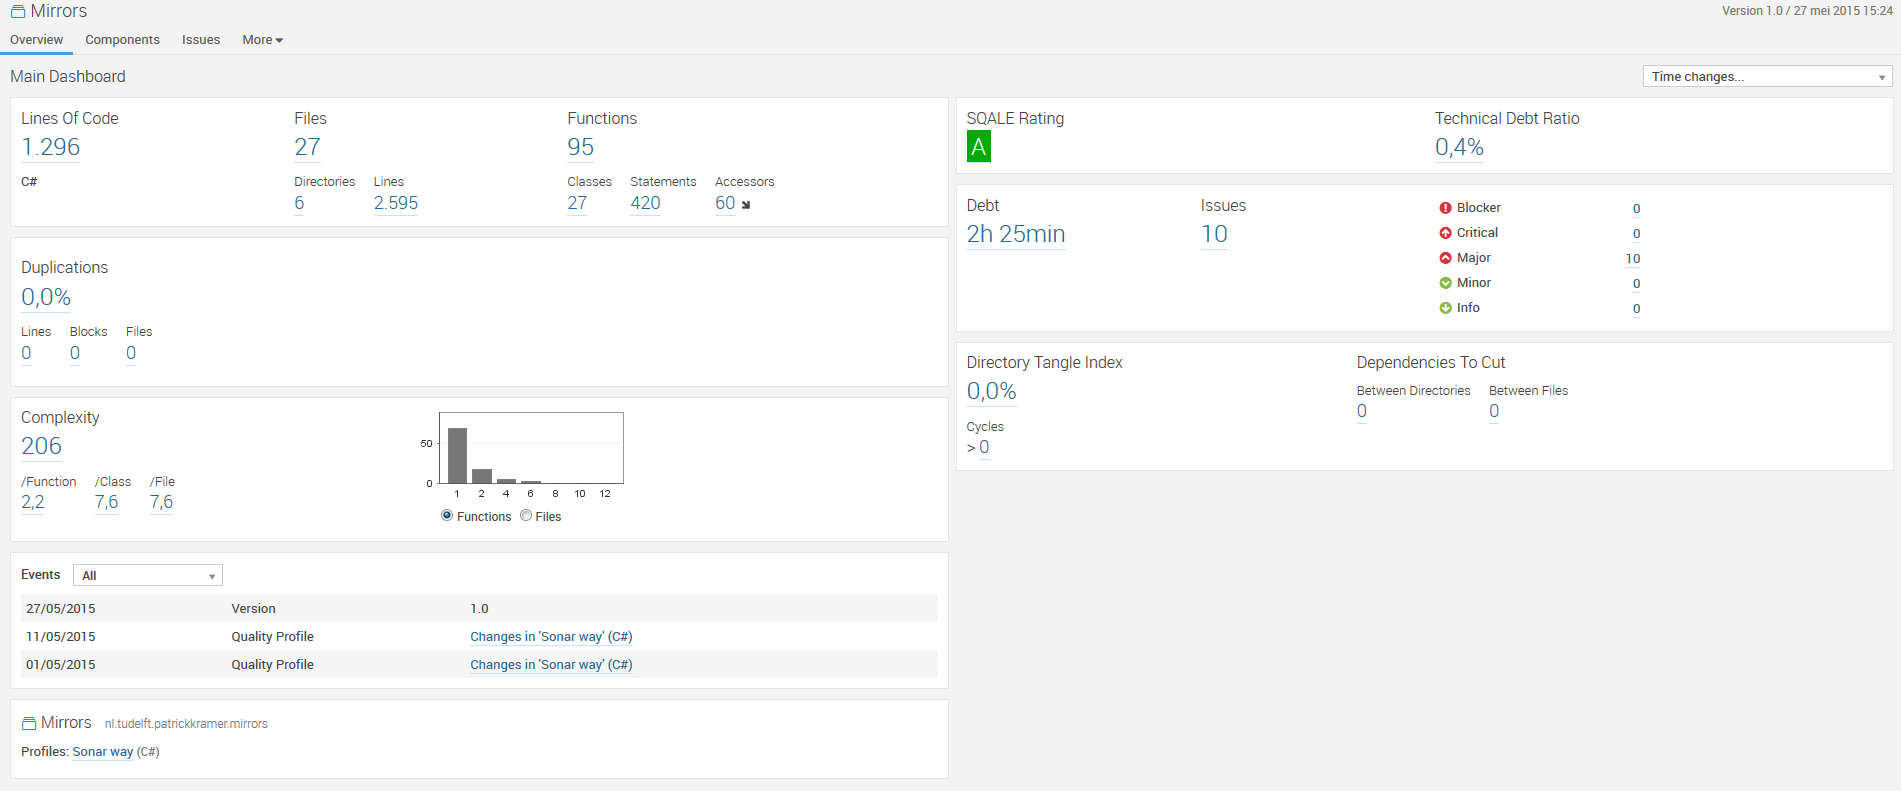
\includegraphics[width=\textwidth]{SonarQube}
			\caption{A SonarQube overview.}
			\label{fig:sonarqube}
		\end{figure}
		
		An issue with SonarQube is that, while it has free options for analyzing
		C\# code, it has none of these free options for analyzing C/C++ code,
		because of the preprocessing that can happen in C or C++ (as explained
		in their blog on \url{http://www.sonarqube.org/ccobjective-c-dark-past-bright-future/}).
		For this reason, it is very hard to analyze the C++ code that we use for the
		OpenCV server.
		
	\section{SIG Evaluation} \label{sec:sigevaluation}
		SIG is an acronym which stands for the Software Improvement Group,
		which is a company that is based in Amsterdam. SIG performs code
		analysis to evaluate code quality on a scale from one to five stars,
		and it does so according to the ISO/IEC 25010 model. Code score is 
		based on the maintainability of the code.
		
		During the project, there are two opportunities to deliver the code 
		that we have written to SIG. The first opportunity is at the end of 
		May, and the second is halfway through June. The first opportunity 
		is used as a midterm quality feedback session, for us to get an idea 
		about how good the code is written and what can be done better. The 
		second opportunity is then intended to hand in the improved code, 
		and for us to then get feedback on how well the code has been improved. 
		The improvements in the code also have a weight in the final result 
		for the project.
		
		The midterm and final evaluation reports we received from SIG are added
		as appendices \ref{app:sig1} and \ref{app:sig2}, respectively.
		
	\section{Demo's and playtesting sessions} \label{sec:demos}
		%TODO Write about the demo with the client.
		...
